\documentclass[11pt]{beamer}
\usetheme{simple}
\setbeamertemplate{footline}{} 
\usepackage{tikz}
\usepackage{sansmathaccent}
\pdfmapfile{+sansmathaccent.map}
\usepackage{pgfplots}
\usepackage{amsmath, amssymb, amsthm}   

%\pgfplotsset{ every non boxed y axis/.append style={y axis line style=-}}
\setbeamertemplate{navigation symbols}{}
\begin{document}
\begin{frame}

\tikzset{every picture/.style={line width=0.75pt}} %set default line width to 0.75pt        

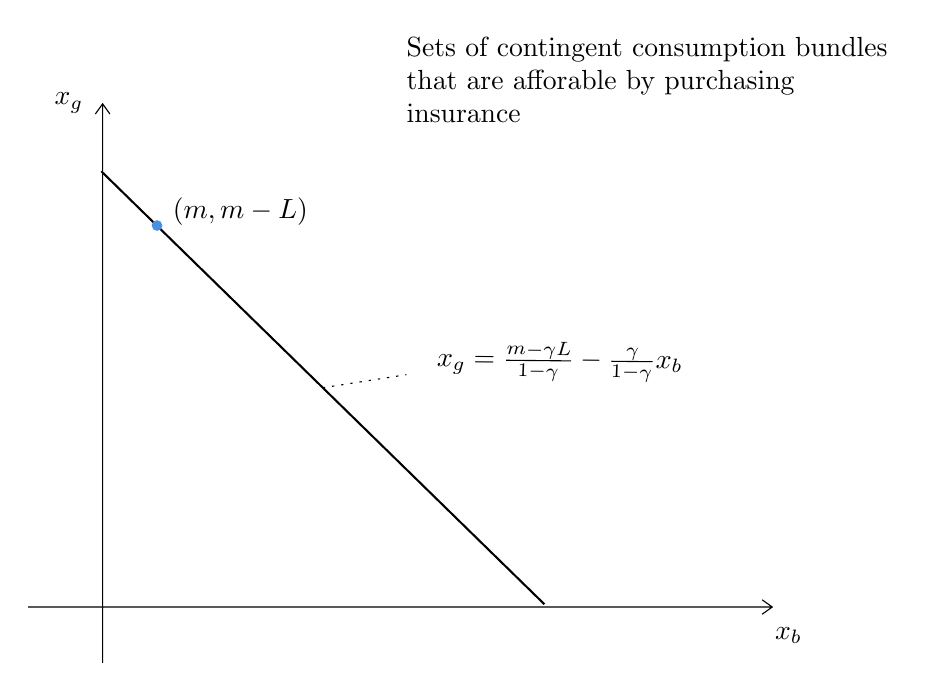
\begin{tikzpicture}[x=0.75pt,y=0.75pt,yscale=-.7,xscale=.7]
%uncomment if require: \path (0,443); %set diagram left start at 0, and has height of 443

%Shape: Axis 2D [id:dp3991482376662687] 
\draw  (74,382.93) -- (586.09,382.93)(125.21,36.6) -- (125.21,421.41) (579.09,377.93) -- (586.09,382.93) -- (579.09,387.93) (120.21,43.6) -- (125.21,36.6) -- (130.21,43.6)  ;
%Straight Lines [id:da1654344051931811] 
\draw [line width=0.75]    (124.28,83.03) -- (429.28,381.03) ;


%Shape: Circle [id:dp6490632364348066] 
\draw  [draw opacity=0][fill={rgb, 255:red, 74; green, 144; blue, 226 }  ,fill opacity=1 ] (158.97,120.35) .. controls (158.97,118.32) and (160.61,116.67) .. (162.65,116.67) .. controls (164.68,116.67) and (166.33,118.32) .. (166.33,120.35) .. controls (166.33,122.39) and (164.68,124.03) .. (162.65,124.03) .. controls (160.61,124.03) and (158.97,122.39) .. (158.97,120.35) -- cycle ;
%Straight Lines [id:da8727541988151988] 
\draw  [dash pattern={on 0.84pt off 2.51pt}]  (276.78,232.03) -- (334.28,223.03) ;



% Text Node
\draw (597.35,402.33) node   {$x_{b}$};
% Text Node
\draw (220,111) node   {$( m,m-L)$};
% Text Node
\draw (102,36) node   {$x_{g}$};
% Text Node
\draw (440,214) node [rotate=-0.56,xslant=0.03]  {$x_{g} =\frac{m-\gamma L}{1-\gamma } -\frac{\gamma }{1-\gamma } x_{b}$};
% Text Node
\draw (500,20) node  [align=left] { Sets of contingent consumption bundles\\  that are afforable by purchasing \\ insurance};
\end{tikzpicture}
\end{frame}
\end{document}